\documentclass[tikz]{standalone}
\usetikzlibrary{shapes,arrows.meta}
\begin{document}
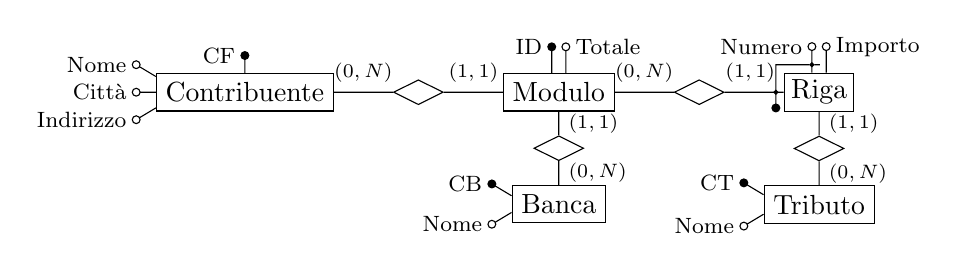
\begin{tikzpicture}
    \draw

    %%* Attributi:
    %%  node[draw, circle, inner sep=1pt, fill=black]{}node[right]{\footnotesize A}
    %%? Distanza orizzontale: E -(0.25,0.x)- A
    %%? Distanza verticale: E -(0,x * 0.22)- A

    %%* Cardinalità:
    %%  node[below right]{\scriptsize $(0,N)$}
    %%  node[above right]{\scriptsize $(0,N)$}
    %%  node[midway, above]{\scriptsize $(0,N)$}

    %%* Relazione:
    %%  node[draw, diamond, shape aspect=2, inner sep=3pt, anchor=90](r1){}
    %%  node[draw, diamond, shape aspect=2, inner sep=0.2pt, anchor=180](r2){R2}

    %%* Entità:
    %%  node[draw, rectangle, anchor=90](e1){}
    %%? Distanza verticale: E -(0.3)- R -(0.3) E
    %%? Distanza orizzontale: E -(0.75)- R -(0.75)- E

    %%* Contribuente
    (0,0)node[draw, rectangle, anchor=90](e1){Contribuente}
    (e1.0)--++(0.75,0)node[draw, diamond, shape aspect=2, inner sep=3pt, anchor=180](r1){}node[midway, above]{\scriptsize $(0,N)$}

    
    (e1.170)--++(-0.25,0.15) node[draw, circle, inner sep=1pt, fill=white]{}node[left]{\footnotesize Nome}
    (e1.180)--++(-0.25,0)node[draw, circle, inner sep=1pt, fill=white]{}node[left]{\footnotesize Città}
    (e1.190)--++(-0.25,-0.15)node[draw, circle, inner sep=1pt, fill=white]{}node[left]{\footnotesize Indirizzo}
    (e1.90)--++(0,0.22)node[draw, circle, inner sep=1pt, fill=black]{}node[left]{\footnotesize CF}

    %%* Modulo
    (r1.0)--++(0.75,0)node[midway, above]{\scriptsize $(1,1)$}node[draw, rectangle, anchor=180](e2){Modulo}
    (e2.0)--++(0.75,0)node[draw, diamond, shape aspect=2, inner sep=3pt, anchor=180](r2){}node[midway, above]{\scriptsize $(0,N)$}
    (e2.270)--++(0,-0.3)node[draw, diamond, shape aspect=2, inner sep=3pt, anchor=90](r3){}node[midway, right]{\scriptsize $(1,1)$}
    
    (e2.110)--++(0,0.33)node[draw, circle, inner sep=1pt, fill=black]{}node[left]{\footnotesize ID}
    (e2.70)--++(0,0.33)node[draw, circle, inner sep=1pt, fill=white]{}node[right]{\footnotesize Totale}

    %%* Banca
    (r3.270)--++(0,-0.3)node[draw, rectangle, anchor=90](e4){Banca}node[midway, right]{\scriptsize $(0,N)$}

    
    (e4.170)--++(-0.25,0.15) node[draw, circle, inner sep=1pt, fill=black]{}node[left]{\footnotesize CB}
    (e4.190)--++(-0.25,-0.15)node[draw, circle, inner sep=1pt, fill=white]{}node[left]{\footnotesize Nome}

    %%* Riga
    (r2.0)--++(0.65,0)node[midway, above]{\scriptsize $(1,1)$}node[draw, circle, inner sep=0.5pt, fill=black](a){}--++(0.1,0)node[draw, rectangle, anchor=180, inner sep=2.5pt](e5){Riga}
    (e5.270)--++(0,-0.3)node[draw, diamond, shape aspect=2, inner sep=3pt, anchor=90](r4){}node[midway, right]{\scriptsize $(1,1)$}

    
    (e5.110)--++(0,0.1)node[draw, circle, inner sep=0.5pt, fill=black](b){}--++(0,0.23)node[draw, circle, inner sep=1pt, fill=white]{}node[left]{\footnotesize Numero}
    (e5.70)--++(0,0.33)node[draw, circle, inner sep=1pt, fill=white]{}node[right]{\footnotesize Importo}

    (a)++(0,-.2)node[draw, circle, inner sep=1pt, fill=black]{}|-(b)--++(0.1,0)

    
    %%* Tributo
    (r4.270)--++(0,-0.3)node[draw, rectangle, anchor=90](e6){Tributo}node[midway, right]{\scriptsize $(0,N)$}

    
    (e6.170)--++(-0.25,0.15) node[draw, circle, inner sep=1pt, fill=black]{}node[left]{\footnotesize CT}
    (e6.190)--++(-0.25,-0.15)node[draw, circle, inner sep=1pt, fill=white]{}node[left]{\footnotesize Nome}



    ;
\end{tikzpicture}
\end{document}